\setlength{\footskip}{8mm}

\chapter{Results and Evaluation}
\label{ch:results}

\section{Evaluation Overview}

This chapter reports the final evidence collected for the inference-time motion-editing pipeline. The evaluation is centered on the apple translation example because it is the only example for which the complete source image, mask, flow support, cached latents, generated outputs, diagnostic arrays, and fixed-seed repeated runs are locally available. The experiment therefore supports a focused case study rather than a broad benchmark across object categories.

The final apple evaluation contains five method variants and three random seeds, giving fifteen runs in total. The variants are designed to answer the central examination question: if the final apple is produced by geometric movement, inpainting, and source-object compositing, what measurable contribution does RAFT-guided diffusion make?

\section{Implemented ML Behavior}

The implementation confirms that the pretrained models are coupled in one differentiable inference graph. At each DDIM step, the U-Net produces conditional and unconditional noise estimates, classifier-free guidance combines them, the VAE decodes a clean-image estimate, and RAFT predicts dense motion relative to the source. PyTorch autograd then differentiates the weighted flow and color energy with respect to the current latent. No Stable Diffusion, CLIP, VAE, or RAFT parameter is updated.

The sampler also preserves source information outside the edit region by replacing latent values with cached or forward-noised source latents. Spatial gradient weighting changes the strength of the external ML signal inside and outside the editable support, while gradient clipping bounds unusually large updates. These mechanisms operate directly on the inference trajectory rather than on the final pixels.

For contained translation, the implementation saves three image states: the decoded diffusion output, the pre-composite output after preservation, and the final output. This separation is important because the final full-pipeline image may use deterministic source-object compositing.

\section{Apple Ablation Protocol}

The apple experiment uses the prompt \emph{an apple on a wooden table}, the source folder \path{./data/apple}, the rightward object support, and a primitive translation of $d_x=150$, $d_y=0$. Each stochastic diffusion variant is run with seeds 0, 1, and 2. The main settings are 120 DDIM steps, classifier-free guidance scale 7.5, guidance weight 30 for RAFT-guided variants, gradient clipping at 60, one recursive step, one RAFT iteration, and fp32 precision.

The five evaluated variants are:

\begin{enumerate}
  \item \textbf{warp-inpaint-only:} deterministic primitive translation, source-hole restoration, and final compositing, with diffusion sampling skipped;
  \item \textbf{original Motion Guidance:} file-based dense-flow guidance without the new primitive initialization and without final compositing;
  \item \textbf{diffusion without RAFT guidance:} primitive hard-warp initialization, source preservation, and zero motion-guidance weight;
  \item \textbf{diffusion with RAFT guidance:} primitive hard-warp initialization, source preservation, and RAFT guidance, but no final composite;
  \item \textbf{full pipeline:} primitive hard-warp initialization, RAFT guidance, source preservation, restoration, and final compositing.
\end{enumerate}

The generated outputs and metadata are stored under \path{backend/results/core_ablation}. Each sample stores the raw diffusion image, pre-composite image, final image, manifest file, and diagnostic arrays for total energy, flow loss, color loss, noise norm, and guidance norm.

\section{Quantitative Results}

Table~\ref{tab:apple-ablation-metrics} summarizes the mean over three seeds. Lower values are better for flow loss, total energy, and background preservation error. Higher sharpness is generally preferable, but it must be interpreted with the visual result because compositing can produce a sharp object while also increasing boundary contrast.

\begin{table}[p]
  \centering
  \tiny
  \caption{Apple ablation results averaged over three seeds. The deterministic baseline has no diffusion loss trajectory because sampling is skipped.}
  \label{tab:apple-ablation-metrics}
  \renewcommand{\arraystretch}{1.12}
  \begin{tabular}{p{1.1in}|p{0.52in}|p{0.62in}|p{0.62in}|p{0.68in}|p{0.73in}|p{0.65in}}
    \hline
    \textbf{Variant} & \textbf{Final source} & \textbf{Total energy} & \textbf{Flow loss} & \textbf{Best flow} & \textbf{Preserve L1} & \textbf{Runtime} \\ \hline \hline
    Warp-inpaint only & Composite & -- & -- & -- & 0.0008 & 2.84 s \\ \hline
    Original Motion Guidance & Diffusion & 48.74 & 15.40 & 9.48 & 0.0065 & 170.71 s \\ \hline
    Diffusion, no RAFT & Diffusion & 30.57 & 8.46 & 8.16 & 0.0136 & 173.83 s \\ \hline
    Diffusion + RAFT & Diffusion & 21.86 & 5.80 & 3.07 & 0.0080 & 175.67 s \\ \hline
    Full pipeline & Composite & 21.71 & 5.67 & 3.13 & 0.0008 & 176.11 s \\ \hline
  \end{tabular}
\end{table}

The main numerical result is that RAFT guidance improves the pre-composite diffusion process. Compared with the no-RAFT diffusion variant, RAFT reduces the final flow loss from 8.46 to 5.80, a reduction of approximately 31 percent. It reduces the best recorded flow loss from 8.16 to 3.07, a reduction of approximately 62 percent. It also reduces the final total guidance energy from 30.57 to 21.86, a reduction of approximately 29 percent. Background preservation error improves from 0.0136 to 0.0080 in the diffusion-only comparison.

These numbers support the claim that RAFT guidance contributes measurable optimization pressure during diffusion. They do not prove that RAFT is solely responsible for the final visually best apple image, because the final full-pipeline result applies deterministic compositing.

\section{Diagnostic Trajectories}

Figure~\ref{fig:apple-flow-loss} plots the recorded RAFT flow loss over logged guidance steps. The RAFT-guided diffusion variants consistently descend below the no-RAFT variant. The original file-flow baseline has higher final flow loss and more instability near the end of sampling. The full pipeline follows the same guided-diffusion behavior as the RAFT variant before its final compositing stage.

\begin{figure}[p]
  \centering
  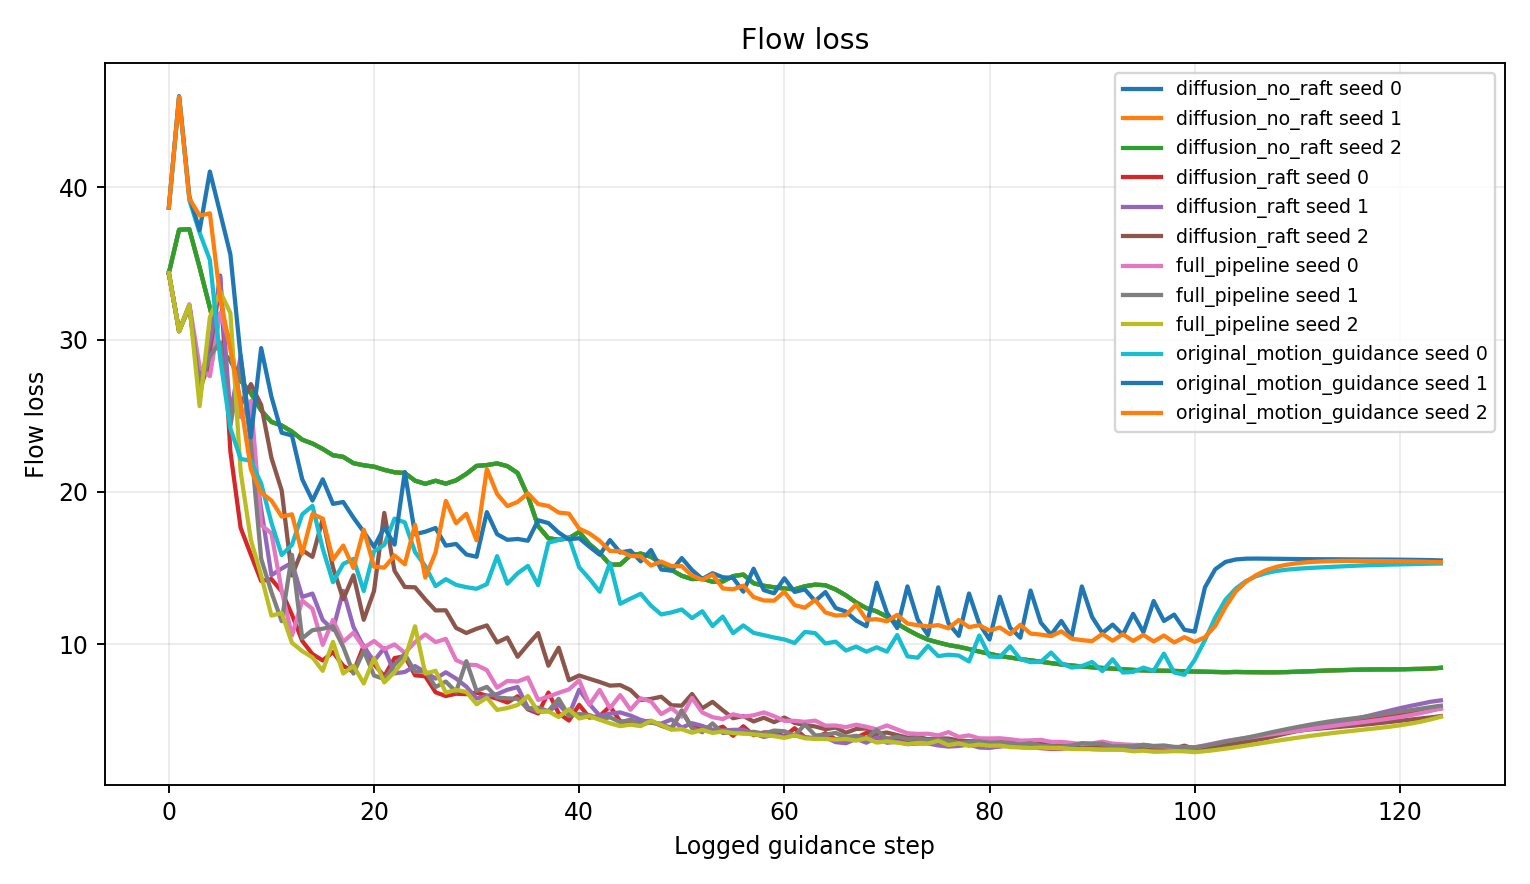
\includegraphics[width=5.8in]{figures/apple_ablation_flow_loss.png}
  \caption{Recorded flow-loss trajectories for the apple ablation. RAFT-guided primitive diffusion reaches lower flow loss than the no-RAFT variant across the three seeds.}
  \label{fig:apple-flow-loss}
\end{figure}

Figure~\ref{fig:apple-total-energy} shows the corresponding total guidance energy. The same pattern appears: RAFT-guided primitive diffusion reaches lower energy than no-RAFT diffusion. These curves are the strongest evidence that RAFT contributes to the diffusion trajectory itself.

\begin{figure}[p]
  \centering
  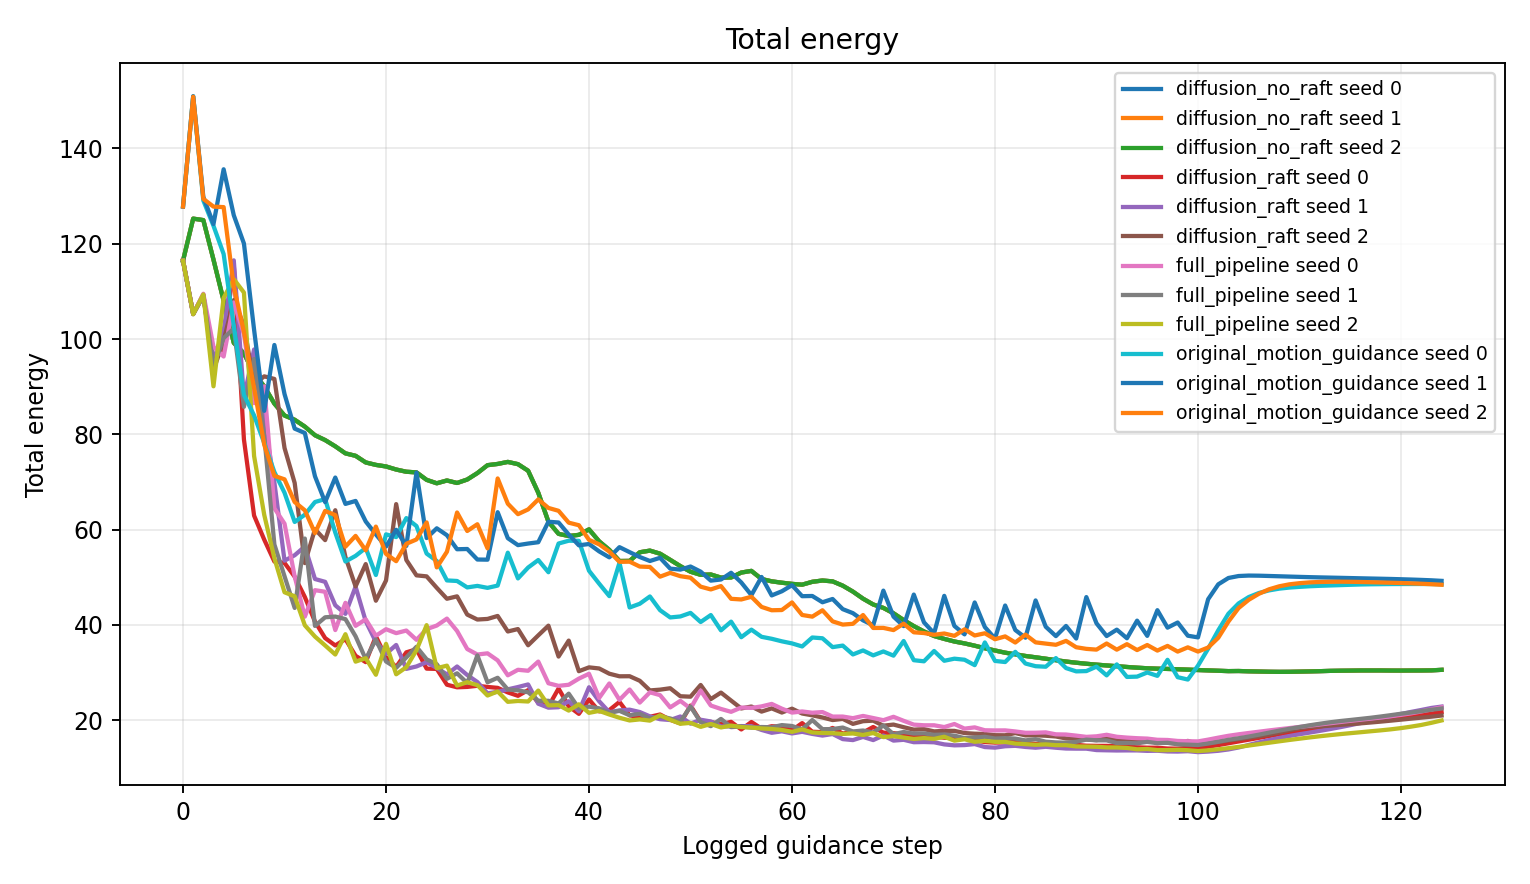
\includegraphics[width=5.8in]{figures/apple_ablation_total_energy.png}
  \caption{Total guidance-energy trajectories for the apple ablation. RAFT-guided variants have lower final energy than the no-RAFT diffusion condition.}
  \label{fig:apple-total-energy}
\end{figure}

\section{Visual Results}

Figure~\ref{fig:apple-final-grid} shows final saved outputs for all variants and seeds. Rows correspond to seeds 0, 1, and 2. Columns show warp-inpaint-only, original Motion Guidance, diffusion without RAFT, diffusion with RAFT, and the full pipeline. The full pipeline produces the most visually coherent final apple across the three seeds. However, the deterministic warp-inpaint-only output is also visually strong, and both of these variants apply final compositing.

\begin{figure}[p]
  \centering
  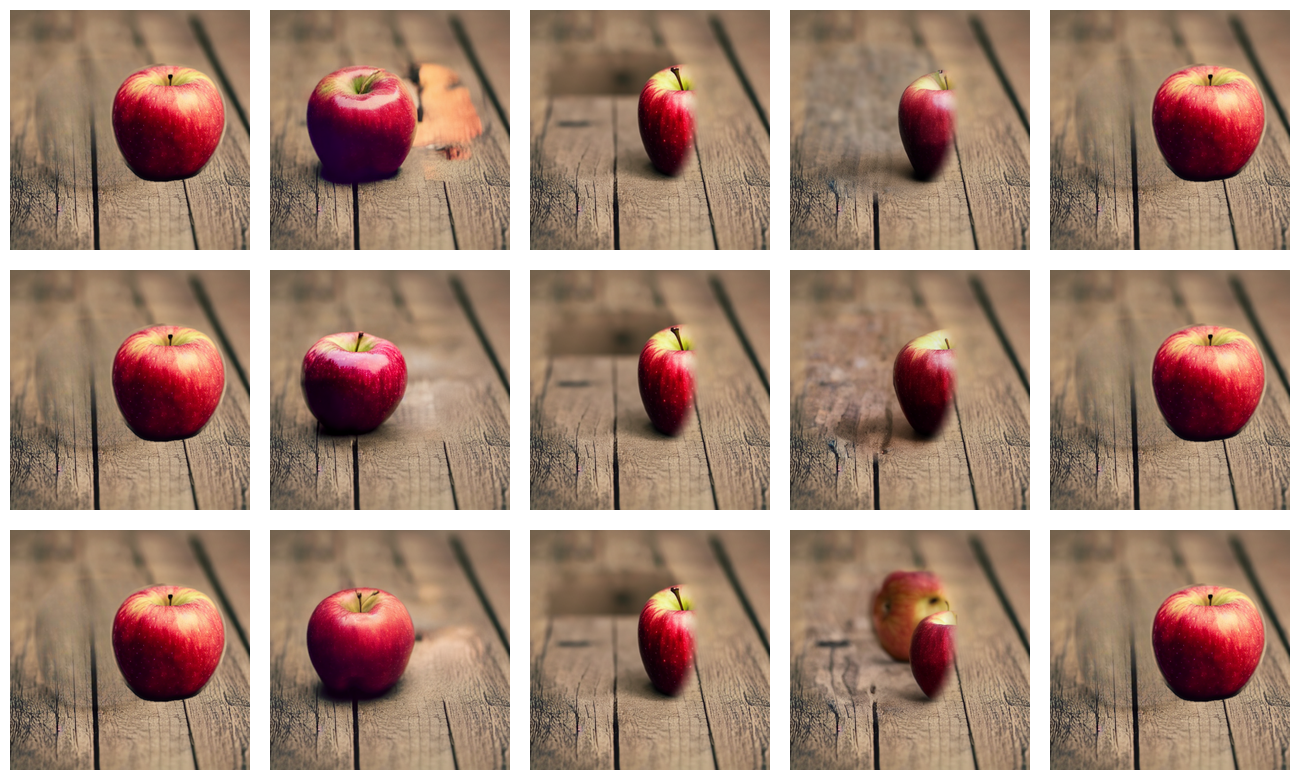
\includegraphics[width=5.9in]{figures/apple_ablation_final_grid.png}
  \caption{Final saved apple outputs. Rows are seeds 0--2. Columns are warp-inpaint-only, original Motion Guidance, diffusion without RAFT, diffusion with RAFT, and full pipeline. The full pipeline is visually strong, but its final image is composited.}
  \label{fig:apple-final-grid}
\end{figure}

Figure~\ref{fig:apple-pre-composite-grid} isolates the pre-composite diffusion outputs for the primitive diffusion variants. This figure is more appropriate for judging the diffusion stage itself. The no-RAFT condition preserves a partial object but does not convincingly complete the edit. RAFT-guided outputs generally align better with the intended motion according to the metrics, but they remain visually incomplete in some seeds. This supports a careful interpretation: RAFT helps the optimization objective, but restoration and compositing are still needed for the final contained-translation result.

\begin{figure}[p]
  \centering
  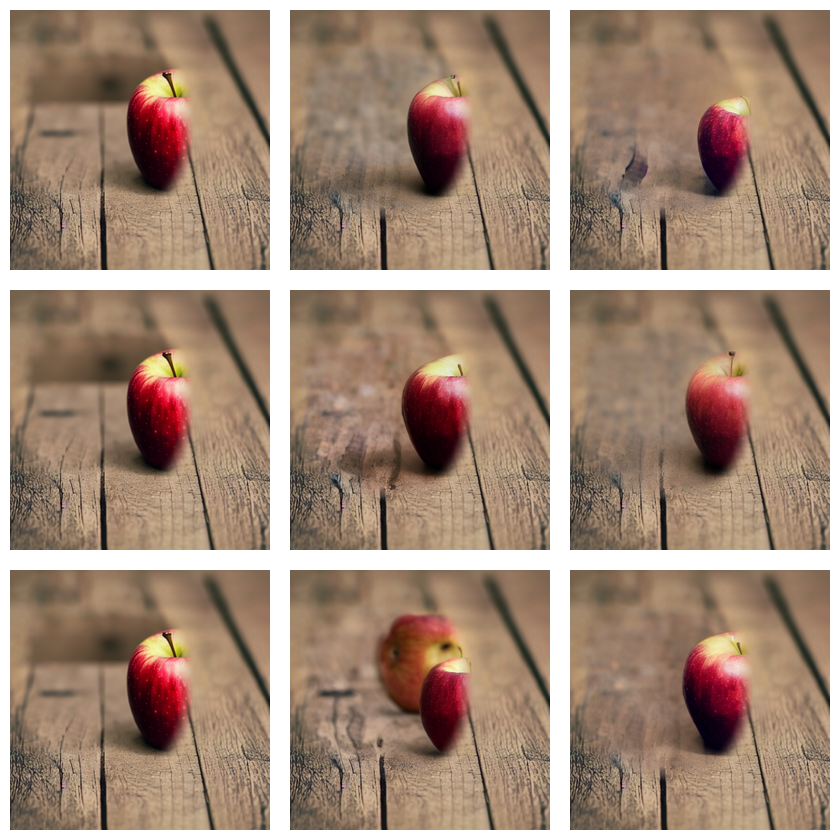
\includegraphics[width=5.7in]{figures/apple_ablation_pre_composite_grid.png}
  \caption{Pre-composite apple outputs for primitive diffusion variants. Rows are seeds 0--2. Columns are no-RAFT diffusion, RAFT-guided diffusion, and full-pipeline pre-composite output. These images separate diffusion behavior from final compositing.}
  \label{fig:apple-pre-composite-grid}
\end{figure}

\section{Answer to the RAFT Contribution Question}

The most important result is the distinction between optimization contribution and final rendering contribution. RAFT-guided diffusion measurably improves the intermediate diffusion process: it reduces final flow loss, best flow loss, total guidance energy, and background preservation error relative to the no-RAFT diffusion variant. Therefore, RAFT is not merely decorative in the code; it changes the measured diffusion trajectory.

At the same time, the final visually best apple image is not produced by diffusion alone. For contained translation, the full pipeline uses deterministic source-object compositing after diffusion. The final image therefore demonstrates the complete hybrid renderer, not an isolated diffusion result. The defensible claim is:

\begin{quote}
RAFT guidance improves the pre-composite diffusion trajectory. Deterministic restoration and compositing produce the cleanest final contained-translation image.
\end{quote}

\section{Additional Generated Cases}

After the apple ablation, two additional real generated cases were run with three seeds each. These runs do not replace the controlled apple ablation, because they do not isolate RAFT versus no-RAFT conditions. They are included to address the concern that the thesis contained only one inspectable result and to show how the implementation behaves outside the main apple translation scene.

The teapot case uses primitive downward translation with final compositing enabled. It is the closest additional example to the apple setting. The tree case uses the available file-based squeeze flow and therefore saves the pre-composite diffusion result as the final image. It is better interpreted as a challenging non-rigid or file-flow stress case rather than as a polished translation result.

\begin{table}[p]
  \centering
  \scriptsize
  \caption{Additional generated cases averaged over three seeds. These results broaden the qualitative evidence but are not controlled component ablations.}
  \label{tab:additional-generated-results}
  \renewcommand{\arraystretch}{1.12}
  \begin{tabular}{p{0.72in}|p{0.82in}|p{0.72in}|p{0.58in}|p{0.58in}|p{0.66in}|p{0.66in}}
    \hline
    \textbf{Case} & \textbf{Motion} & \textbf{Final source} & \textbf{Flow loss} & \textbf{Best flow} & \textbf{Preserve L1} & \textbf{Runtime} \\ \hline \hline
    Teapot & Translate down & Composite & 4.23 $\pm$ 0.14 & 3.09 $\pm$ 0.16 & 0.0005 $\pm$ 0.0000 & 170.86 $\pm$ 1.50 s \\ \hline
    Tree & File-flow squeeze & Diffusion & 3.65 $\pm$ 0.39 & 2.02 $\pm$ 0.14 & 0.0014 $\pm$ 0.0004 & 172.68 $\pm$ 3.28 s \\ \hline
  \end{tabular}
\end{table}

Figure~\ref{fig:teapot-extra-grid} shows the teapot runs. The final images are stable across seeds because the contained-translation path applies restoration and source-object compositing after diffusion, as in the full apple pipeline.

\begin{figure}[p]
  \centering
  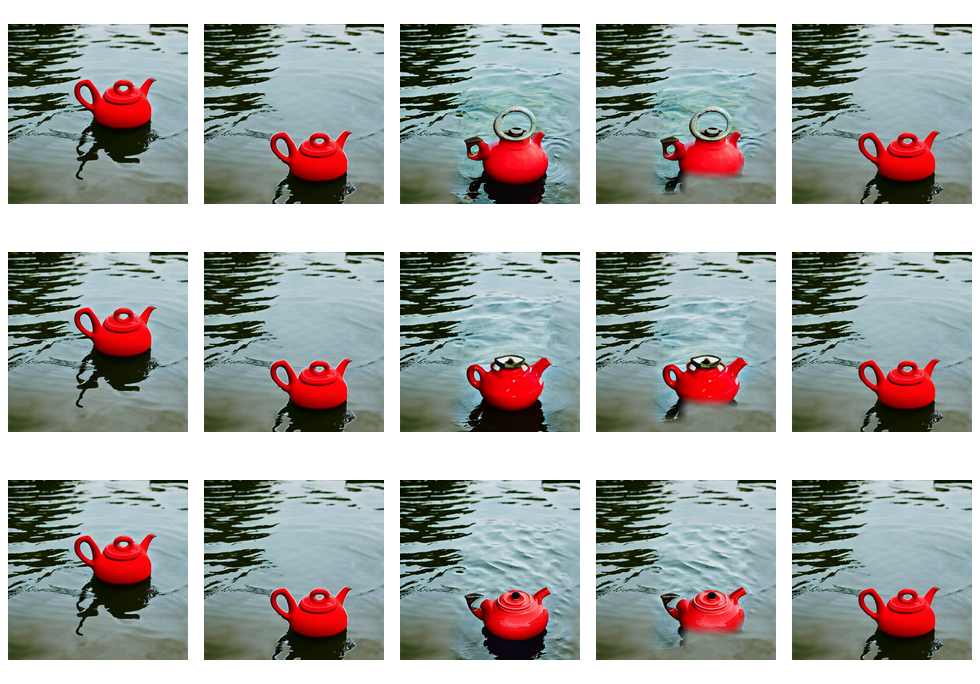
\includegraphics[width=5.9in]{figures/teapot_full_pipeline_grid.png}
  \caption{Additional teapot translation case over three seeds. Columns show source, warped initialization, decoded diffusion output, and final composited output.}
  \label{fig:teapot-extra-grid}
\end{figure}

Figure~\ref{fig:tree-extra-grid} shows the tree runs. Seed 2 is visually the most coherent. Seeds 0 and 1 show noticeable variation in crown shape and texture, which supports the thesis limitation that non-rigid or file-flow edits remain less reliable than contained rigid translations.

\begin{figure}[p]
  \centering
  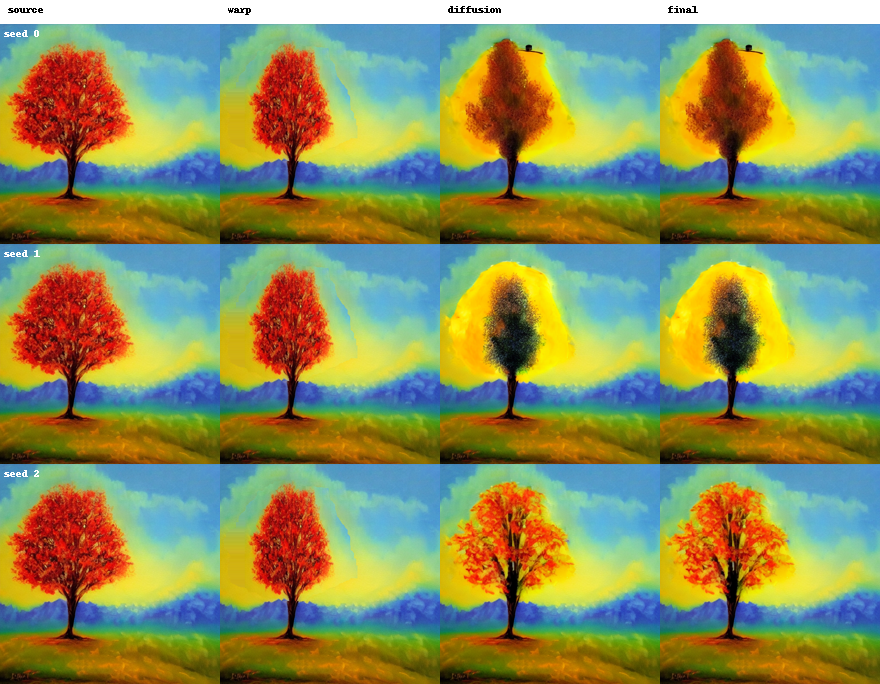
\includegraphics[width=5.9in]{figures/tree_full_pipeline_grid.png}
  \caption{Additional tree file-flow squeeze case over three seeds. This case is useful as a stress test; it should not be presented as a polished rigid-translation result.}
  \label{fig:tree-extra-grid}
\end{figure}

\section{Status of Other Examples}

Table~\ref{tab:main-generated-results} distinguishes the evaluated apple ablation and additional generated cases from configured or presentation examples. A configured preset is not counted as an evaluated result unless its complete output artifacts are available for inspection.

\begin{table}[t]
  \caption{Summary of examples and evidence status.}
  \centering
  \small
  \begin{tabular}{p{0.8in}|p{1.0in}|p{1.3in}|p{1.85in}}
    \hline
    Example & Motion & Output Type & Evaluation Summary \\ \hline \hline
    Apple & Translate right & 15-run ablation & Primary controlled quantitative and qualitative evidence. \\ \hline
    Teapot & Translate down & 3 generated seeds & Additional contained-translation evidence; final image uses compositing. \\ \hline
    Tree & File-flow squeeze & 3 generated seeds & Additional stress case; non-rigid/file-flow behavior is less stable. \\ \hline
    Lion & Translate left & Smoke test only & Excluded from main results because the object support touches the image boundary and clips during translation. \\ \hline
    Woman & Non-rigid & Shipped asset mode & Excluded from evaluation. \\ \hline
    Topiary & Non-rigid & Shipped asset mode & Excluded from evaluation. \\ \hline
  \end{tabular}
  \label{tab:main-generated-results}
\end{table}

\section{Evaluation Summary}

The evaluation supports five conclusions. First, the complete pipeline can produce a stable contained rightward apple translation across three seeds. Second, RAFT-guided primitive diffusion improves the measured diffusion trajectory compared with no-RAFT diffusion. Third, original file-flow Motion Guidance performs worse than the primitive RAFT-guided variants on this apple setup. Fourth, additional teapot and tree runs broaden the inspectable evidence, but they are not controlled ablations. Fifth, the final visual quality of contained translation is dominated by restoration and compositing, so the thesis must not claim that diffusion alone creates the final apple or teapot result.

The evidence remains narrow. The only full component ablation covers one object category, one background, one translation magnitude, one mask, one RAFT-iteration setting, and three seeds. The additional teapot and tree cases reduce the single-result weakness, but they do not establish broad generalization or state-of-the-art superiority.

\FloatBarrier
